\documentclass{standalone}

\usepackage{tikz}
\usetikzlibrary{angles,quotes}
\usepackage{amsmath,amssymb,amsfonts}

\usepackage{pgfplots}
\definecolor{darkgreen}{rgb}{0.0, 0.42, 0.24}
\definecolor{amethyst}{rgb}{0.6, 0.4, 0.8}

\pgfplotsset{compat=newest}
\pgfplotsset{every axis/.append style={
                     tick label style={font=\footnotesize},
                 }}


\begin{document}
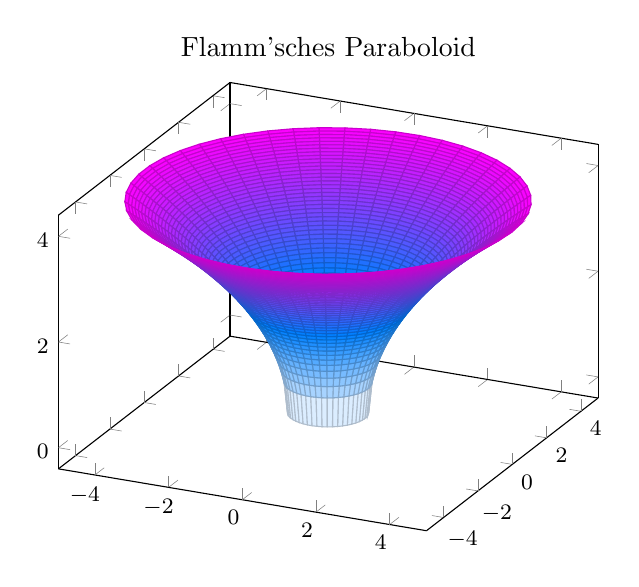
\begin{tikzpicture}
    \begin{axis}[title=$\text{Flamm'sches Paraboloid}$,colormap/cool,
    data cs=polar,
    domain=0:360,y domain=1:5,
    samples=50,
    declare function={
       flamm(\r)={2*sqrt(\r-1)};
       pol2cartX(\angle,\radius) = \radius * cos(\angle);
       pol2cartY(\angle,\radius) = \radius * sin(\angle);
       }]
       \addplot3[surf,z buffer=sort]{flamm(y)};
    \end{axis}
\end{tikzpicture} 
\end{document}